% Figure 1: the length-coupling taxonomy, drawn in TikZ so that it shares the
% body font and stays vector at any zoom.
\begin{figure}[t]
\centering
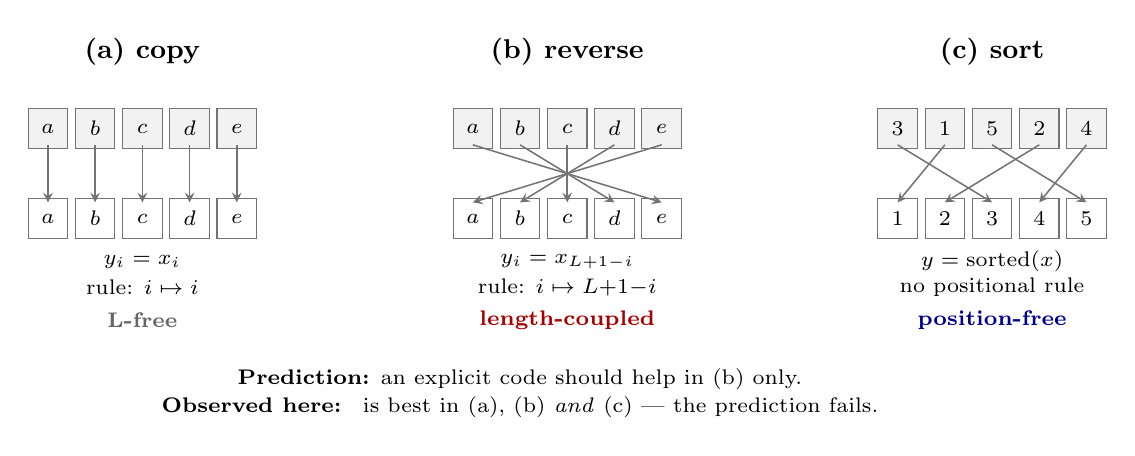
\begin{tikzpicture}[
  x=1cm, y=1cm, scale=1.09, transform shape,
  cell/.style={draw=black!55, fill=black!5, minimum width=4.6mm,
               minimum height=4.6mm, inner sep=0pt, font=\scriptsize},
  outcell/.style={cell, fill=white},
  conn/.style={->, >=stealth, draw=black!55, line width=0.55pt},
  ttl/.style={font=\small\bfseries},
  rule/.style={font=\scriptsize},
  cls/.style={font=\scriptsize\bfseries},
  note/.style={font=\scriptsize, align=center},
  arr/.style={->, >=stealth, draw=black!55, line width=0.6pt}
]

% ---------------- (a) copy ----------------
\begin{scope}[xshift=0cm]
  \node[ttl] at (1.1,1.95) {(a) copy};
  \foreach \i/\t in {0/a,1/b,2/c,3/d,4/e}{
    \node[cell] at (\i*0.55,1.05) {$\t$};
    \node[outcell] at (\i*0.55,0.00) {$\t$};
    \draw[conn] (\i*0.55,0.86) -- (\i*0.55,0.19);
  }
  \node[rule] at (1.1,-0.50) {$y_i = x_i$};
  \node[rule] at (1.1,-0.80) {rule: $i \mapsto i$};
  \node[cls, text=black!60] at (1.1,-1.18) {L-free};
\end{scope}

% ---------------- (b) reverse ----------------
\begin{scope}[xshift=4.95cm]
  \node[ttl] at (1.1,1.95) {(b) reverse};
  \foreach \i/\t in {0/a,1/b,2/c,3/d,4/e}{
    \node[cell] at (\i*0.55,1.05) {$\t$};
    \node[outcell] at (\i*0.55,0.00) {$\t$};
  }
  \draw[conn] (0.00,0.86) -- (2.20,0.19);
  \draw[conn] (0.55,0.86) -- (1.65,0.19);
  \draw[conn] (1.10,0.86) -- (1.10,0.19);
  \draw[conn] (1.65,0.86) -- (0.55,0.19);
  \draw[conn] (2.20,0.86) -- (0.00,0.19);
  \node[rule] at (1.1,-0.50) {$y_i = x_{L+1-i}$};
  \node[rule] at (1.1,-0.80) {rule: $i \mapsto L{+}1{-}i$};
  \node[cls, text=red!65!black] at (1.1,-1.18) {length-coupled};
\end{scope}

% ---------------- (c) sort ----------------
\begin{scope}[xshift=9.90cm]
  \node[ttl] at (1.1,1.95) {(c) sort};
  \foreach \i/\t in {0/3,1/1,2/5,3/2,4/4}{
    \node[cell] at (\i*0.55,1.05) {$\t$};
  }
  \foreach \i/\t in {0/1,1/2,2/3,3/4,4/5}{
    \node[outcell] at (\i*0.55,0.00) {$\t$};
  }
  \draw[conn] (0.55,0.86) -- (0.00,0.19);
  \draw[conn] (1.65,0.86) -- (0.55,0.19);
  \draw[conn] (0.00,0.86) -- (1.10,0.19);
  \draw[conn] (2.20,0.86) -- (1.65,0.19);
  \draw[conn] (1.10,0.86) -- (2.20,0.19);
  \node[rule] at (1.1,-0.50) {$y = \mathrm{sorted}(x)$};
  \node[rule] at (1.1,-0.80) {no positional rule};
  \node[cls, text=blue!55!black] at (1.1,-1.18) {position-free};
\end{scope}

% ---------------- verdict strip ----------------
\node[note, anchor=north] at (5.5,-1.62)
  {\textbf{Prediction:} an explicit code should help in (b) only.};
\node[note, anchor=north] at (5.5,-1.95)
  {\textbf{Observed here:} \nope{} is best in (a), (b) \emph{and} (c) --- the prediction fails.};

\end{tikzpicture}
\caption{The axis we test. A task is \emph{length-coupled} when the rule mapping
an output position to the input positions it reads is written in terms of the
sequence length $L$; (b) is coupled because the rule contains $L$, while (a) uses
the same rule at every $L$. Panel (c) shows why a coarse ``local vs.\ global''
distinction would fail: sorting reads the whole input, yet has no positional rule
at all, since which input supplies output $i$ is decided by the values. Our
hypothesis was that an explicit position code should matter only in (b); the
experiments in \secref{sec:results} contradict it.}
\label{fig:taxonomy}
\end{figure}
